\documentclass[12pt]{article}

\usepackage{../thesis}

\usepackage{tikz} 

\begin{document}

\pagestyle{empty}

\begin{tikzpicture}
    \node[anchor=south west,inner sep=0,rotate=0.6] (image) at (0,0) {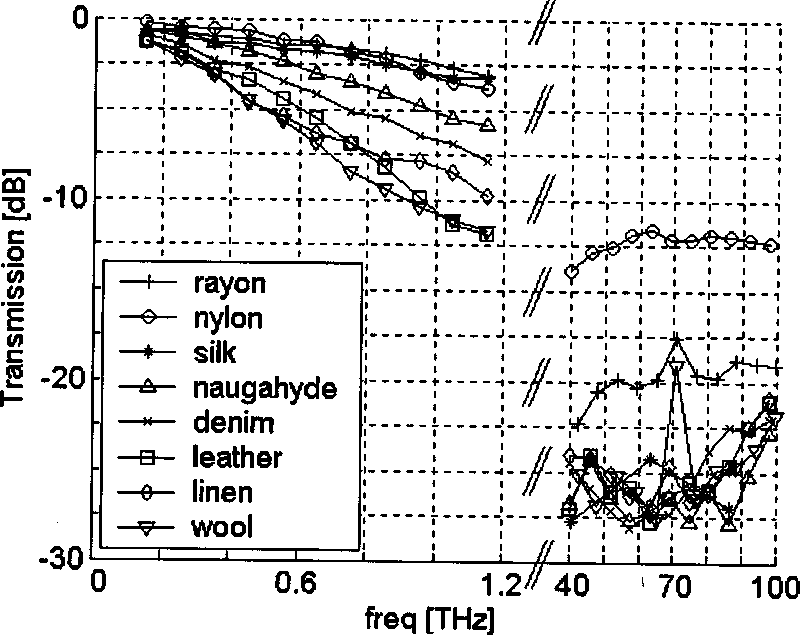
\includegraphics[width=4.0in]{../images/ch1-clothes-bjarnason.png}};
    \begin{scope}[x={(image.south east)},y={(image.north west)}]
	    %\draw[help lines,xstep=.1,ystep=.1] (0,0) grid (1.0,1);
		%\foreach \x in {0,1,...,9} { \node [anchor=north] at (\x/10,0) {0.\x}; }
		%\foreach \y in {0,1,...,9} { \node [anchor=east] at (0,\y/10) {0.\y}; }
        
        % f = 0 GHz at 0.1115, f = 1200 GHz at 0.6239.
        % 10 dB band is 318.0 -- 375.9 GHz
		
        \draw[black,fill=blue!50,opacity=0.6] (0.2473, 0.6) rectangle (0.2720, 0.973) node[below right] {};

        % \draw[black,rotate=-0.6] (0.1115,0) -- (0.1115,1.00) node[midway,right] {}; % scale bar
        % \draw[black,rotate=-0.6] (0.6239,0) -- (0.6239,1.00) node[midway,right] {}; % scale bar
    \end{scope}
\end{tikzpicture}

\end{document}
